\documentclass[11pt,a4paper]{article}
%%%%%%%%%%%%%%%%%%%%%%%%% Credit %%%%%%%%%%%%%%%%%%%%%%%%

% template ini dibuat oleh martin.manullang@if.itera.ac.id untuk dipergunakan oleh seluruh sivitas akademik itera.

%%%%%%%%%%%%%%%%%%%%%%%%% PACKAGE starts HERE %%%%%%%%%%%%%%%%%%%%%%%%
\usepackage{graphicx}
\usepackage{caption}
\usepackage{microtype}
\captionsetup[table]{name=Tabel}
\captionsetup[figure]{name=Gambar}
\usepackage{tabulary}
\usepackage{minted}
\usepackage{amsmath}
\usepackage{fancyhdr}
\usepackage{amssymb}
\usepackage{amsthm}
\usepackage{placeins}
\usepackage{amsfonts}
\usepackage{graphicx}
\usepackage[all]{xy}
\usepackage{tikz}
\usepackage{verbatim}
\usepackage[left=2cm,right=2cm,top=3cm,bottom=2.5cm]{geometry}
\usepackage{hyperref}
\hypersetup{
    colorlinks,
    linkcolor={red!50!black},
    citecolor={blue!50!black},
    urlcolor={blue!80!black}
}
\usepackage{caption}
\usepackage{float}
\usepackage{subcaption}
\usepackage{multirow}
\usepackage{psfrag}
\usepackage{lmodern}
\usepackage[T1]{fontenc}
\usepackage[scaled]{beramono}
% Enable inserting code into the document
\usepackage{listings}
\usepackage{xcolor} 
% custom color & style for listing
\definecolor{codegreen}{rgb}{0,0.6,0}
\definecolor{codegray}{rgb}{0.5,0.5,0.5}
\definecolor{codepurple}{rgb}{0.58,0,0.82}
\definecolor{backcolour}{rgb}{0.95,0.95,0.92}
\definecolor{LightGray}{gray}{0.9}
\lstdefinestyle{mystyle}{
	backgroundcolor=\color{backcolour},   
	commentstyle=\color{green},
	keywordstyle=\color{codegreen},
	numberstyle=\tiny\color{codegray},
	stringstyle=\color{codepurple},
	basicstyle=\ttfamily\footnotesize,
	breakatwhitespace=false,         
	breaklines=true,                 
	captionpos=b,                    
	keepspaces=true,                 
	numbers=left,                    
	numbersep=5pt,                  
	showspaces=false,                
	showstringspaces=false,
	showtabs=false,                  
	tabsize=2
}
\lstset{style=mystyle}
\renewcommand{\lstlistingname}{Kode}
%%%%%%%%%%%%%%%%%%%%%%%%% PACKAGE ends HERE %%%%%%%%%%%%%%%%%%%%%%%%


%%%%%%%%%%%%%%%%%%%%%%%%% Data Diri %%%%%%%%%%%%%%%%%%%%%%%%
\newcommand{\student}{\textbf{Fawwaz Abhitah Sugiarto (122140014)}}
\newcommand{\course}{\textbf{Sistem Teknologi Multimedia (IF25-40305)}}
\newcommand{\assignment}{\textbf{Worksheet 1: Setup Python Environment untuk Multimedia}}

%%%%%%%%%%%%%%%%%%% using theorem style %%%%%%%%%%%%%%%%%%%%
\newtheorem{thm}{Theorem}
\newtheorem{lem}[thm]{Lemma}
\newtheorem{defn}[thm]{Definition}
\newtheorem{exa}[thm]{Example}
\newtheorem{rem}[thm]{Remark}
\newtheorem{coro}[thm]{Corollary}
\newtheorem{quest}{Question}[section]
%%%%%%%%%%%%%%%%%%%%%%%%%%%%%%%%%%%%%%%%
\usepackage{lipsum}%% a garbage package you don't need except to create examples.
\usepackage{fancyhdr}
\pagestyle{fancy}
\lhead{Fawwaz Abhitah Sugiarto (122140014)}
\rhead{ \thepage}
\cfoot{\textbf{Worksheet 1: Setup Python Environment untuk Multimedia}}
\renewcommand{\headrulewidth}{0.4pt}
\renewcommand{\footrulewidth}{0.4pt}

%%%%%%%%%%%%%%  Shortcut for usual set of numbers  %%%%%%%%%%%

\newcommand{\N}{\mathbb{N}}
\newcommand{\Z}{\mathbb{Z}}
\newcommand{\Q}{\mathbb{Q}}
\newcommand{\R}{\mathbb{R}}
\newcommand{\C}{\mathbb{C}}
\setlength\headheight{14pt}

%%%%%%%%%%%%%%%%%%%%%%%%%%%%%%%%%%%%%%%%%%%%%%%%%%%%%%%555
\begin{document}
\thispagestyle{empty}
\begin{center}
	
\includegraphics[scale = 0.15]{Figure/ifitera-header.png}
	\vspace{0.1cm}
\end{center}
\noindent
\rule{17cm}{0.2cm}\\[0.3cm]
Nama: \student \hfill Tugas Ke: \assignment\\[0.1cm]
Mata Kuliah: \course \hfill Tanggal: \today\\
\rule{17cm}{0.05cm}
\vspace{0.1cm}



%%%%%%%%%%%%%%%%%%%%%%%%%%%%%%%%%%%%%%%%%%%%% BODY DOCUMENT %%%%%%%%%%%%%%%%%%%%%%%%%%%%%%%%%%%%%%%%%%%%%
\section{Tujuan Pembelajaran}
Setelah menyelesaikan worksheet ini, mahasiswa diharapkan mampu:
\begin{itemize}
    \item Memahami pentingnya manajemen environment Python untuk pengembangan multimedia
    \item Menginstall dan mengkonfigurasi Python environment menggunakan conda, venv, atau uv
    \item Menginstall library-library Python yang diperlukan untuk multimedia processing
    \item Memverifikasi instalasi dengan mengimpor dan menguji library multimedia
    \item Mendokumentasikan proses konfigurasi dan hasil pengujian dalam format \LaTeX
\end{itemize}

\section{Latar Belakang}
Python telah menjadi bahasa pemrograman yang sangat populer untuk multimedia processing karena memiliki ekosistem library yang sangat kaya. Namun, untuk dapat bekerja dengan multimedia secara efektif, kita perlu mengatur environment Python dengan benar dan menginstall library-library yang tepat.

Manajemen environment Python sangat penting untuk:
\begin{itemize}
    \item Menghindari konflik antar library (dependency conflict)
    \item Memastikan reproducibility dari project
    \item Memudahkan kolaborasi antar developer
    \item Memisahkan project yang berbeda dengan requirement yang berbeda
\end{itemize}

\section{Instruksi Tugas}

\subsection{Persiapan}
\textbf{Sebelum memulai, pastikan Anda telah:}
\begin{itemize}
    \item Menginstall Python 3.8 atau lebih baru di sistem Anda
    \item Memilih salah satu tool manajemen environment: \textbf{conda}, \textbf{venv}, atau \textbf{uv}
    \item Membuka terminal/command prompt
    \item Menyiapkan dokumen \LaTeX\ ini untuk dokumentasi
\end{itemize}

\subsection{Bagian 1: Membuat Environment Python}
Pilih \textbf{SALAH SATU} dari tiga opsi berikut dan ikuti langkah-langkahnya:

\subsubsection{Opsi 1: Menggunakan Conda (Direkomendasikan untuk pemula)}
Jalankan perintah berikut di terminal:

\begin{lstlisting}[language=bash, caption=Membuat environment dengan Conda]
# Membuat environment baru dengan nama 'multimedia'
conda create -n multimedia python=3.11

# Mengaktifkan environment
conda activate multimedia

# Verifikasi environment aktif
conda info --envs
\end{lstlisting}

\subsubsection{Opsi 2: Menggunakan venv (Built-in Python)}
\begin{lstlisting}[language=bash, caption=Membuat environment dengan venv]
# Membuat environment baru
python3 -m venv multimedia-env

# Mengaktifkan environment (Linux/Mac)
source multimedia-env/bin/activate

# Mengaktifkan environment (Windows)
# multimedia-env\Scripts\activate

# Verifikasi environment aktif
which python
\end{lstlisting}

\subsubsection{Opsi 3: Menggunakan uv (Modern dan cepat)}
\begin{lstlisting}[language=bash, caption=Membuat environment dengan uv]
# Install uv terlebih dahulu jika belum ada
# pip install uv

# Membuat environment baru
uv venv multimedia-uv

# Mengaktifkan environment (Linux/Mac)
source multimedia-uv/bin/activate

# Mengaktifkan environment (Windows)
# multimedia-uv\Scripts\activate

# Verifikasi environment aktif
which python
\end{lstlisting}

\textbf{Dokumentasikan di sini:}
\begin{itemize}
    \item Tool manajemen environment yang Anda pilih: \textbf{[uv]}
    \item Screenshot atau copy-paste output dari perintah verifikasi environment
    \begin{figure}[htbp] 
    \centering
    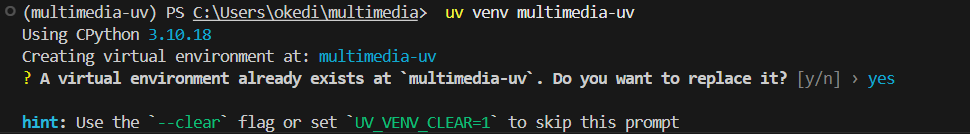
\includegraphics[width=0.7\textwidth]{Figure/ss1.png}
    \caption{Membuat Environment pada Windows}
    \label{fig:contoh-gambar}
    \end{figure}

    \begin{figure}[htbp] 
    \centering
    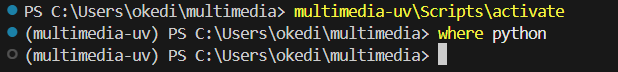
\includegraphics[width=0.7\textwidth]{Figure/ss2.png}
    \caption{Mengaktifkan Environment pada Windows}
    \label{fig:contoh-gambar}
    \end{figure}
\end{itemize}

\subsection{Bagian 2: Instalasi Library Multimedia}
Setelah environment aktif, install library-library berikut:

\subsubsection{Library Audio Processing}
\begin{lstlisting}[language=bash, caption=Instalasi library audio]
# Untuk conda:
conda install -c conda-forge librosa soundfile scipy

# Untuk pip (venv/uv):
pip install librosa soundfile scipy
\end{lstlisting}

\subsubsection{Library Image Processing}
\begin{lstlisting}[language=bash, caption=Instalasi library image]
# Untuk conda:
conda install -c conda-forge opencv pillow scikit-image matplotlib

# Untuk pip (venv/uv):
pip install opencv-python pillow scikit-image matplotlib
\end{lstlisting}

\subsubsection{Library Video Processing}
\begin{lstlisting}[language=bash, caption=Instalasi library video]
# Untuk conda:
conda install -c conda-forge ffmpeg
pip install moviepy

# Untuk pip (venv/uv):
pip install moviepy
\end{lstlisting}

\subsubsection{Library General Purpose}
\begin{lstlisting}[language=bash, caption=Instalasi library umum]
# Untuk conda:
conda install numpy pandas jupyter

# Untuk pip (venv/uv):
pip install numpy pandas jupyter
\end{lstlisting}

\textbf{Dokumentasikan di sini:}
\begin{itemize}
    \item Perintah instalasi yang Anda gunakan
    \begin{enumerate}
        \item pip install librosa soundfile scipy
        \item pip install opencv-python pillow scikit-image matplotlib
        \item pip install moviepy
        \item pip install numpy pandas jupyter
    \end{enumerate}
    \item Screenshot proses instalasi atau output sukses
    \begin{figure}[htbp] 
    \centering
    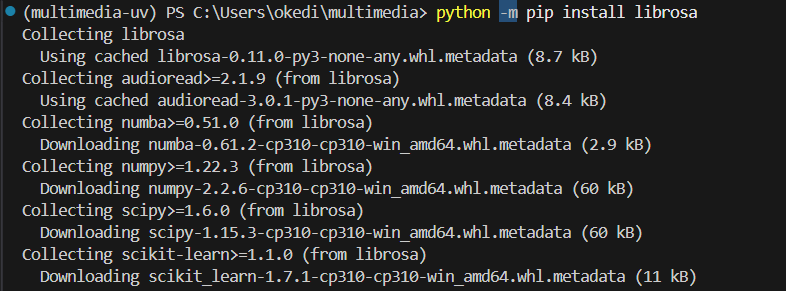
\includegraphics[width=0.7\textwidth]{Figure/ss3.png}
    \caption{Proses Instalasi Library librosa}
    \label{fig:contoh-gambar}
    \end{figure}

    \begin{figure}[htbp]
    \centering
    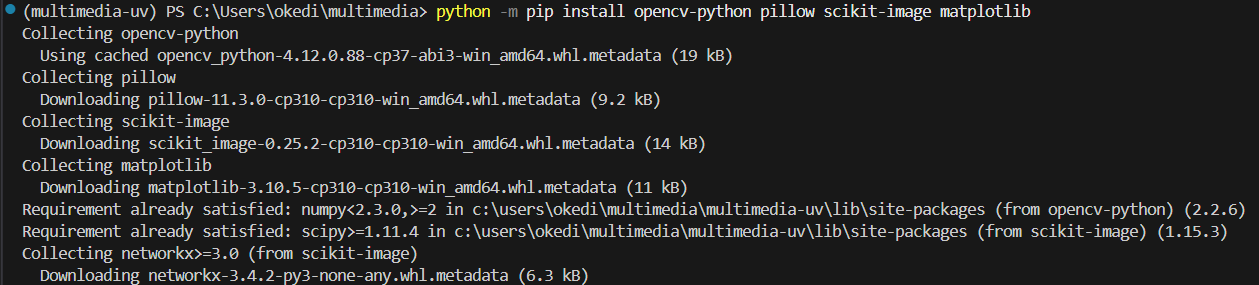
\includegraphics[width=0.7\textwidth]{Figure/ss4.png}
    \caption{Proses Instalasi Library opencv}
    \label{fig:contoh-gambar}
    \end{figure}

    \begin{figure}[htbp]
    \centering
    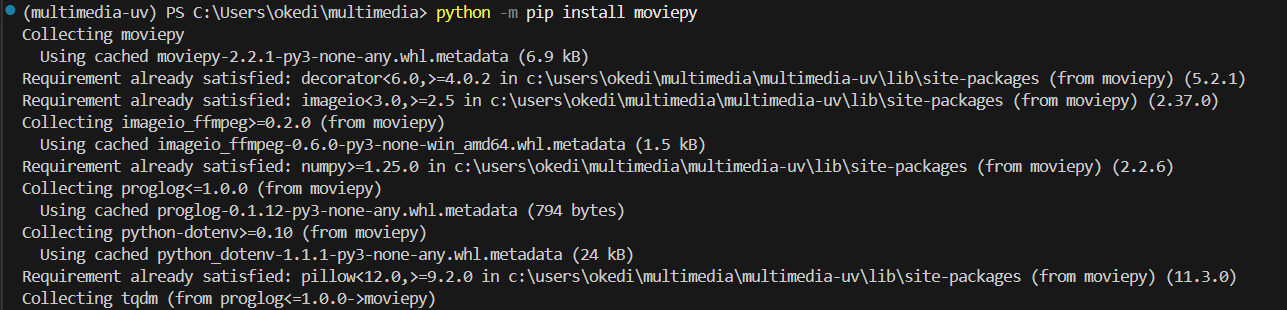
\includegraphics[width=0.7\textwidth]{Figure/ss5.png}
    \caption{Proses Instalasi Library moviepy}
    \label{fig:contoh-gambar}
    \end{figure}

    \begin{figure}[H]
    \centering
    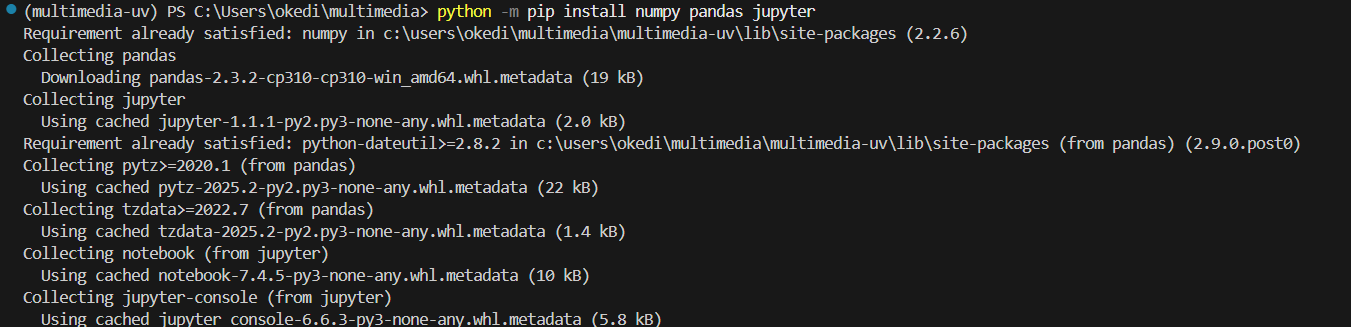
\includegraphics[width=0.7\textwidth]{Figure/ss6.png}
    \caption{Proses Instalasi Library numpy pandas jupyter}
    \label{fig:contoh-gambar}
    \end{figure}
    
    \item Daftar library yang berhasil diinstall dengan versinya
    \begin{itemize}
        \item librosa \, v0.11.0
        \item soundfile \, v0.13.1
        \item scipy \, v1.15.3
        \item cv2 (OpenCV) \, v4.12.0
        \item PIL (Pillow) \, v11.3.0
        \item scikit-image \, v0.25.2
        \item matplotlib \, v3.10.5
        \item moviepy \, v2.1.2
        \item numpy \, v2.2.6
        \item pandas \, v2.3.2
        \item jupyter (notebook) \, v7.4.5
    \end{itemize}

\end{itemize}

\subsection{Bagian 3: Verifikasi Instalasi}
Buat file Python sederhana untuk menguji semua library yang telah diinstall:

\textbf{Jalankan script dan dokumentasikan hasilnya:}
\subsubsection{Verifikasi Instalasi Library Python}
\begin{lstlisting}[language=Python, caption=Verifikasi instalasi library multimedia Python]
print("=== Verifikasi Instalasi Library ===\n")

libraries = [
    ("librosa", "import librosa", "librosa.__version__"),
    ("soundfile", "import soundfile", "soundfile.__version__"),
    ("scipy", "import scipy", "scipy.__version__"),
    ("cv2 (OpenCV)", "import cv2", "cv2.__version__"),
    ("PIL (Pillow)", "from PIL import Image, __version__ as pil_version", "pil_version"),
    ("scikit-image", "import skimage", "skimage.__version__"),
    ("matplotlib", "import matplotlib", "matplotlib.__version__"),
    ("moviepy", "import moviepy", "moviepy.__version__"),
    ("numpy", "import numpy", "numpy.__version__"),
    ("pandas", "import pandas", "pandas.__version__"),
    ("jupyter (notebook)", "import notebook", "notebook.__version__"),
]

for name, statement, version_attr in libraries:
    try:
        exec(statement)
        try:
            version = eval(version_attr)
            print(f"[OK] {name} terinstall (versi: {version})")
        except Exception:
            print(f"[OK] {name} terinstall (versi tidak dapat dideteksi)")
    except Exception as e:
        print(f"[FAIL] {name} gagal di-import -> {e}")

print("\n=== Verifikasi selesai ===")
\end{lstlisting}

\begin{figure}[H] 
    \centering
    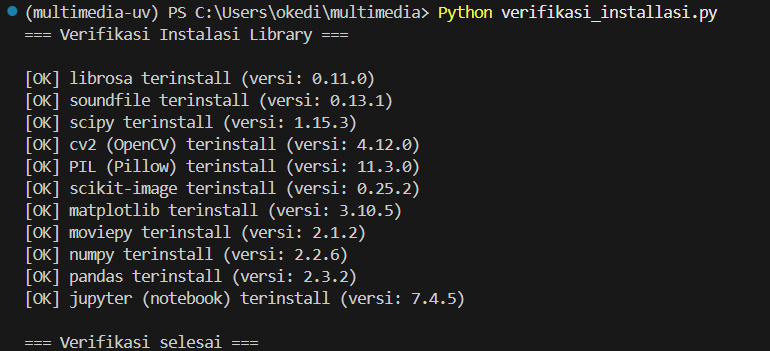
\includegraphics[width=0.7\textwidth]{Figure/verifikasi.png}
    \caption{Output Verifikasi Instalasi Library Multimedia}
    \label{fig:contoh-gambar}
\end{figure}

\subsection{Bagian 4: Simple Test dengan Sample Code}
Buat dan jalankan contoh sederhana untuk setiap kategori multimedia:

\subsubsection{Test Audio Processing}
\begin{lstlisting}[language=Python, caption=Test audio processing sederhana]
import numpy as np
import matplotlib.pyplot as plt

# Generate simple sine wave
duration = 2  # seconds
sample_rate = 44100
frequency = 440  # A4 note

t = np.linspace(0, duration, int(sample_rate * duration))
audio_signal = np.sin(2 * np.pi * frequency * t)

# Plot waveform
plt.figure(figsize=(10, 4))
plt.plot(t[:1000], audio_signal[:1000])  # Plot first 1000 samples
plt.title('Sine Wave (440 Hz)')
plt.xlabel('Time (s)')
plt.ylabel('Amplitude')
plt.grid(True)
plt.savefig('sine_wave_test.png', dpi=150, bbox_inches='tight')
plt.show()

print(f"Generated {duration}s sine wave at {frequency}Hz")
print(f"Sample rate: {sample_rate}Hz")
print(f"Total samples: {len(audio_signal)}")
\end{lstlisting}

\subsubsection{Test Image Processing}
\begin{lstlisting}[language=Python, caption=Test image processing sederhana]
import numpy as np
import matplotlib.pyplot as plt
from PIL import Image

# Create a simple test image
width, height = 400, 300
image = np.zeros((height, width, 3), dtype=np.uint8)

# Add some patterns
image[:, :width//3, 0] = 255  # Red section
image[:, width//3:2*width//3, 1] = 255  # Green section
image[:, 2*width//3:, 2] = 255  # Blue section

# Add a white circle in the center
center_x, center_y = width//2, height//2
radius = 50
Y, X = np.ogrid[:height, :width]
mask = (X - center_x)**2 + (Y - center_y)**2 <= radius**2
image[mask] = [255, 255, 255]

# Display and save
plt.figure(figsize=(8, 6))
plt.imshow(image)
plt.title('Test Image with RGB Stripes and White Circle')
plt.axis('off')
plt.savefig('test_image.png', dpi=150, bbox_inches='tight')
plt.show()

print(f"Created test image: {width}x{height} pixels")
print(f"Image shape: {image.shape}")
print(f"Image dtype: {image.dtype}")
\end{lstlisting}

\textbf{Dokumentasikan hasil eksekusi:}
\begin{itemize}
    \item Screenshot output dari kedua script di atas
    \begin{figure}[H]
    \centering
    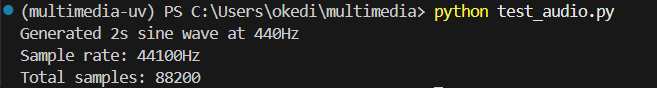
\includegraphics[width=0.7\textwidth]{Figure/ss7.png}
    \caption{Output dari script test audio}
    \label{fig:contoh-gambar}
    \end{figure}
    \begin{figure}[H]
        \centering
        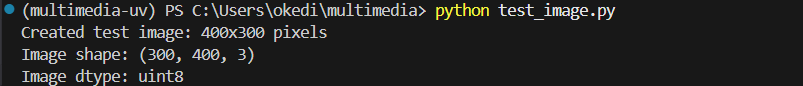
\includegraphics[width=0.7\textwidth]{Figure/ss9.png}
        \caption{Output dari script test image}
        \label{fig:contoh-gambar}
    \end{figure}
    \item Gambar yang dihasilkan (sine\_wave\_test.png dan test\_image.png)
    \begin{figure}[H]
        \centering
        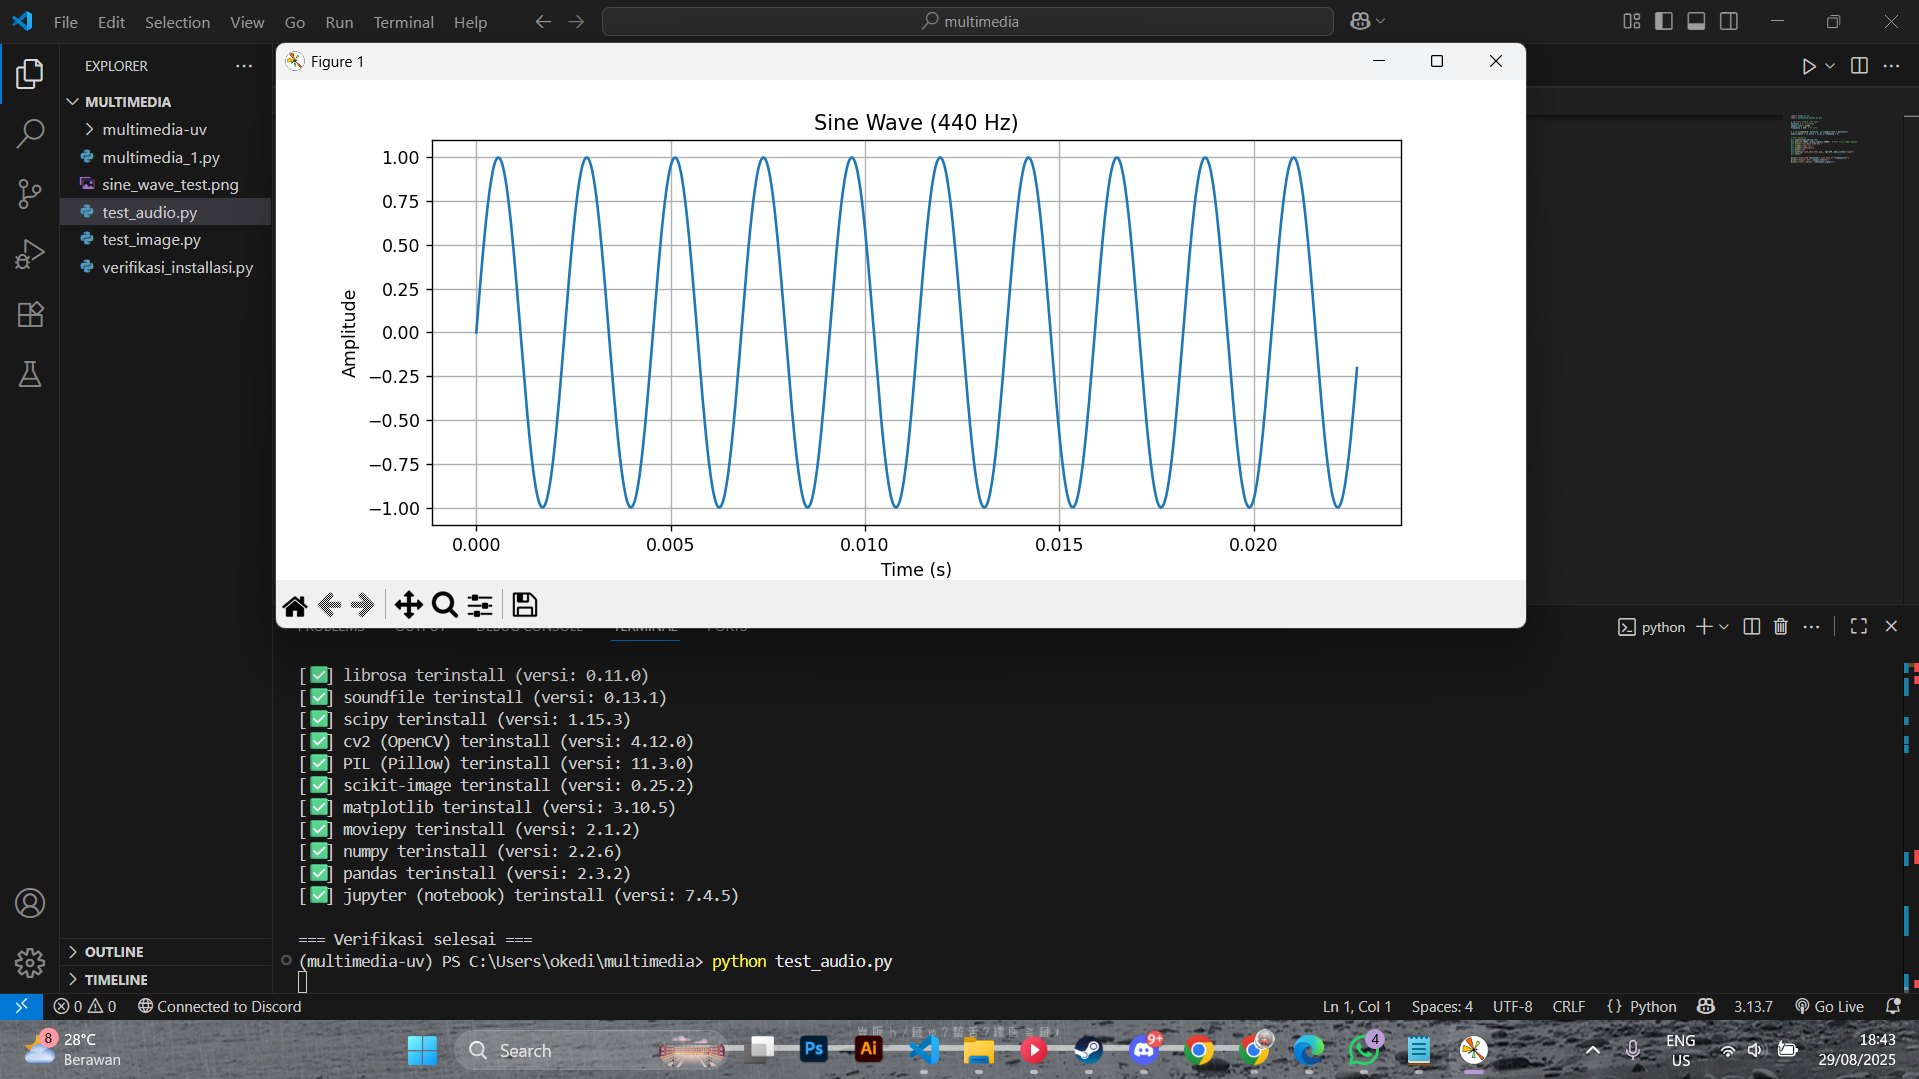
\includegraphics[width=0.7\textwidth]{Figure/ss8.png}
        \caption{Hasil dari script test audio}
        \label{fig:sine_wave_test}
    \end{figure}
    \begin{figure}[H]
        \centering
        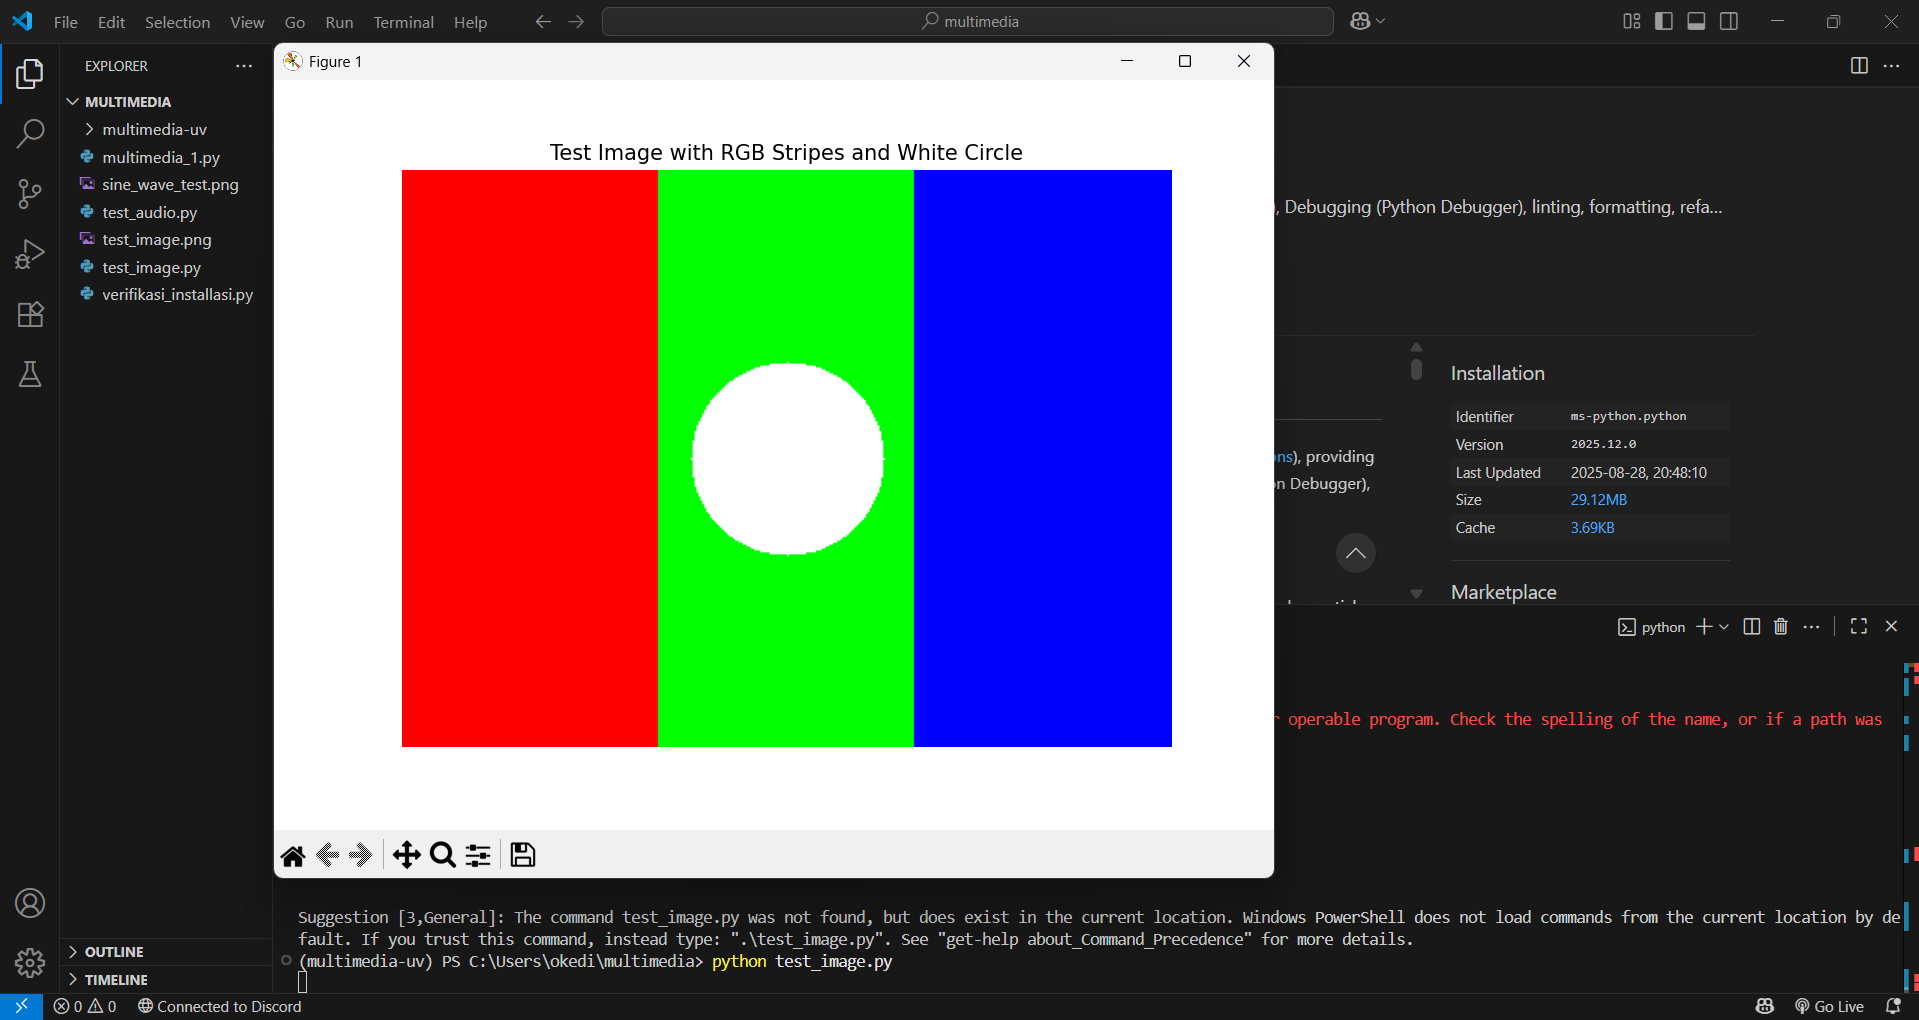
\includegraphics[width=0.7\textwidth]{Figure/ss10.png}
        \caption{Hasil dari script test image RGB}
        \label{fig:test_image}
    \end{figure}
    \item Error message jika ada dan cara mengatasinya
\end{itemize}

\section{Bagian Laporan}

\subsection{Output Verifikasi Instalasi}
\textbf{Copy-paste output lengkap dari script \texttt{verifikasi\_instalasi.py} di sini:}

\begin{lstlisting}[caption=Output verifikasi instalasi]
=== Verifikasi Instalasi Library ===

[OK] librosa terinstall (versi: 0.8.1)
[OK] soundfile terinstall (versi: 0.10.3)
[OK] scipy terinstall (versi: 1.7.1)
[OK] cv2 (OpenCV) terinstall (versi: 4.5.3)
[OK] PIL (Pillow) terinstall (versi: 8.4.0)
[OK] scikit-image terinstall (versi: 0.18.3)
[OK] matplotlib terinstall (versi: 3.4.3)
[OK] moviepy terinstall (versi: 1.0.3)
[OK] numpy terinstall (versi: 1.21.2)
[OK] pandas terinstall (versi: 1.3.3)
[OK] jupyter (notebook) terinstall (versi: 1.0.0)

=== Verifikasi selesai ===
\end{lstlisting}

\subsection{Screenshot Hasil Test}
\textbf{Sisipkan screenshot atau gambar hasil dari:}
\begin{itemize}
    \item Terminal/command prompt yang menunjukkan environment aktif
    \begin{figure}[H]
        \centering
        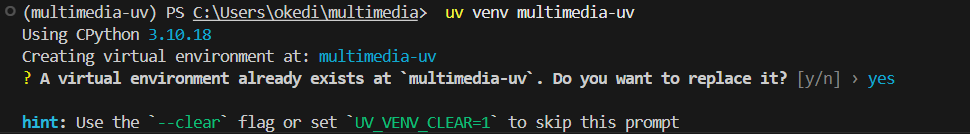
\includegraphics[width=0.7\textwidth]{Figure/ss1.png}
        \caption{Environment aktif di terminal}
        \label{fig:env_aktif}
    \end{figure}
    \item Output dari script test audio (sine wave plot)
    \begin{figure}[H]
        \centering
        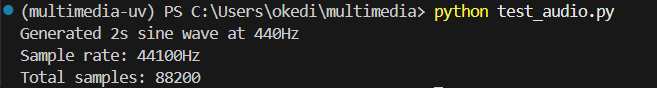
\includegraphics[width=0.7\textwidth]{Figure/ss7.png}
        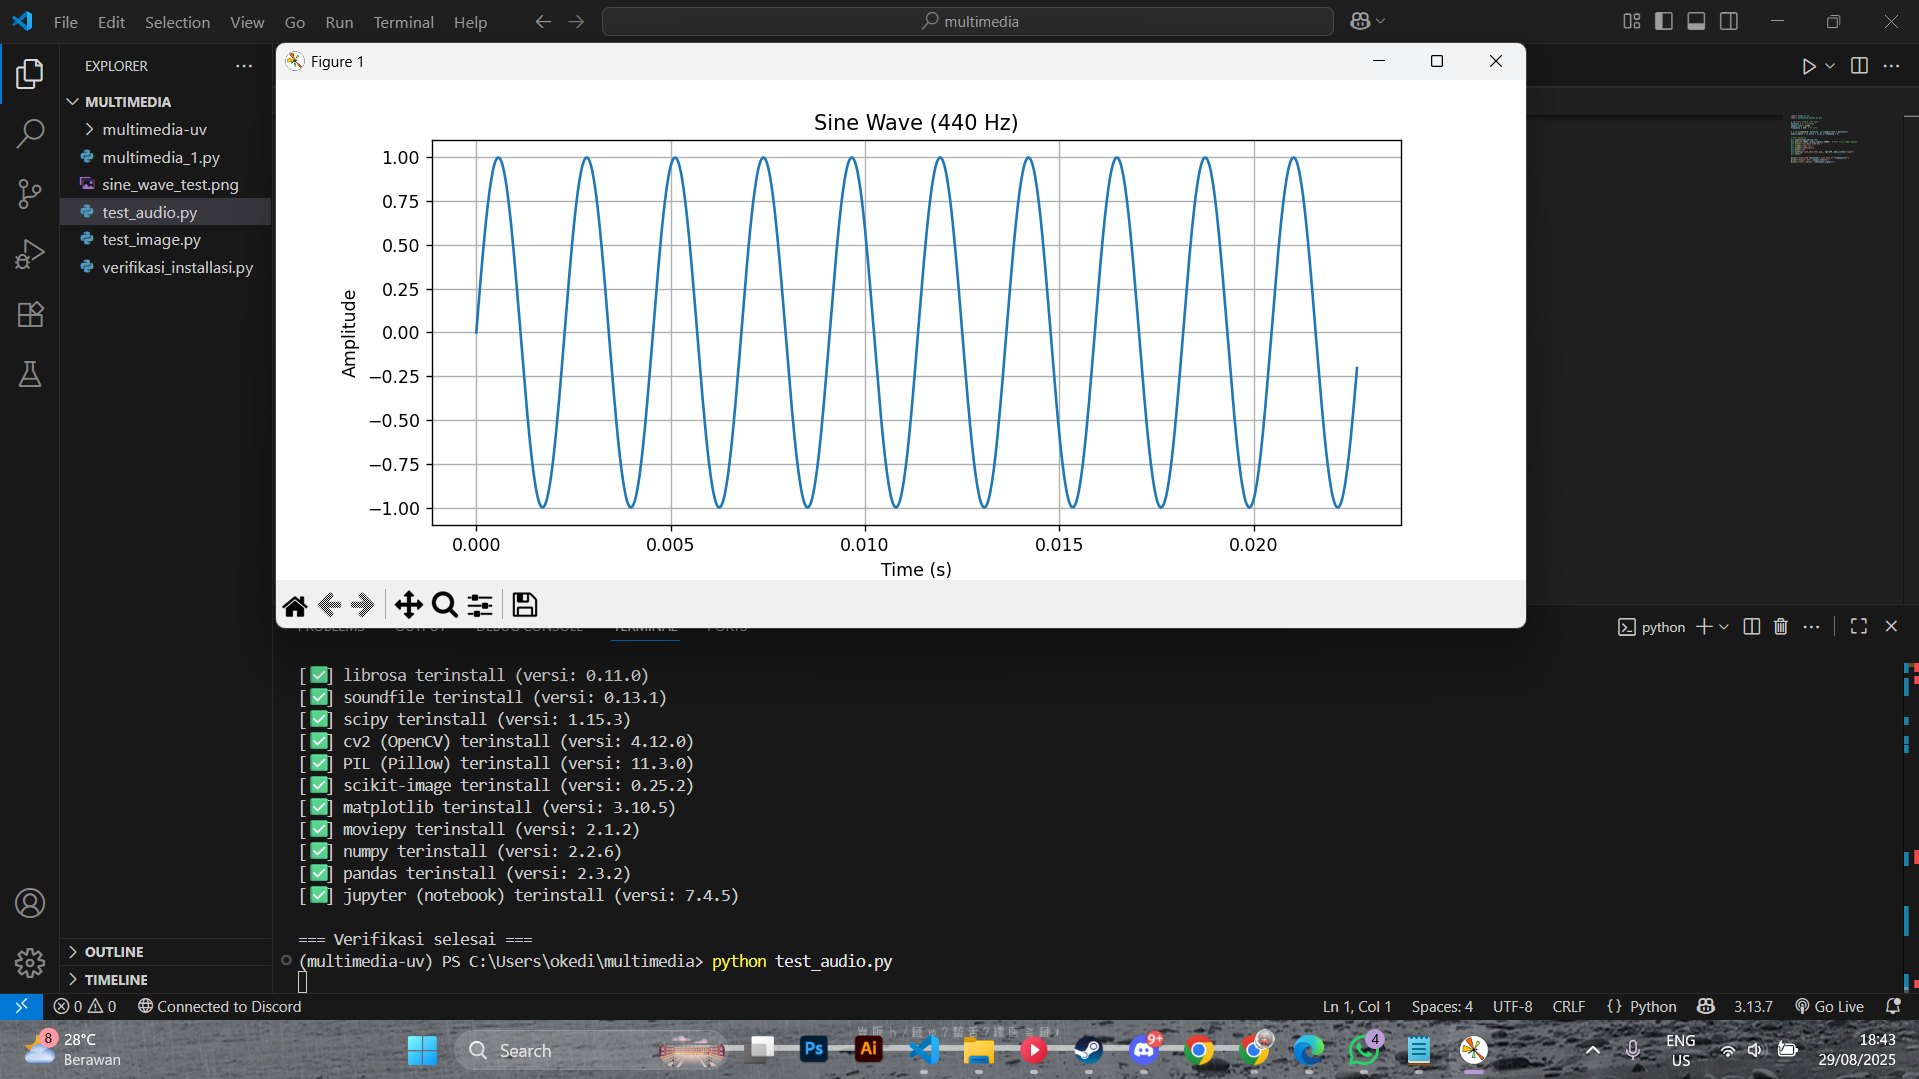
\includegraphics[width=0.7\textwidth]{Figure/ss8.png}
        \caption{Output dari script test audio}
        \label{fig:contoh-gambar}
    \end{figure}
    \item Output dari script test image (RGB stripes dengan circle)
    \begin{figure}[H]
        \centering
        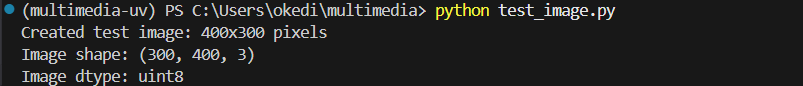
\includegraphics[width=0.7\textwidth]{Figure/ss9.png}
        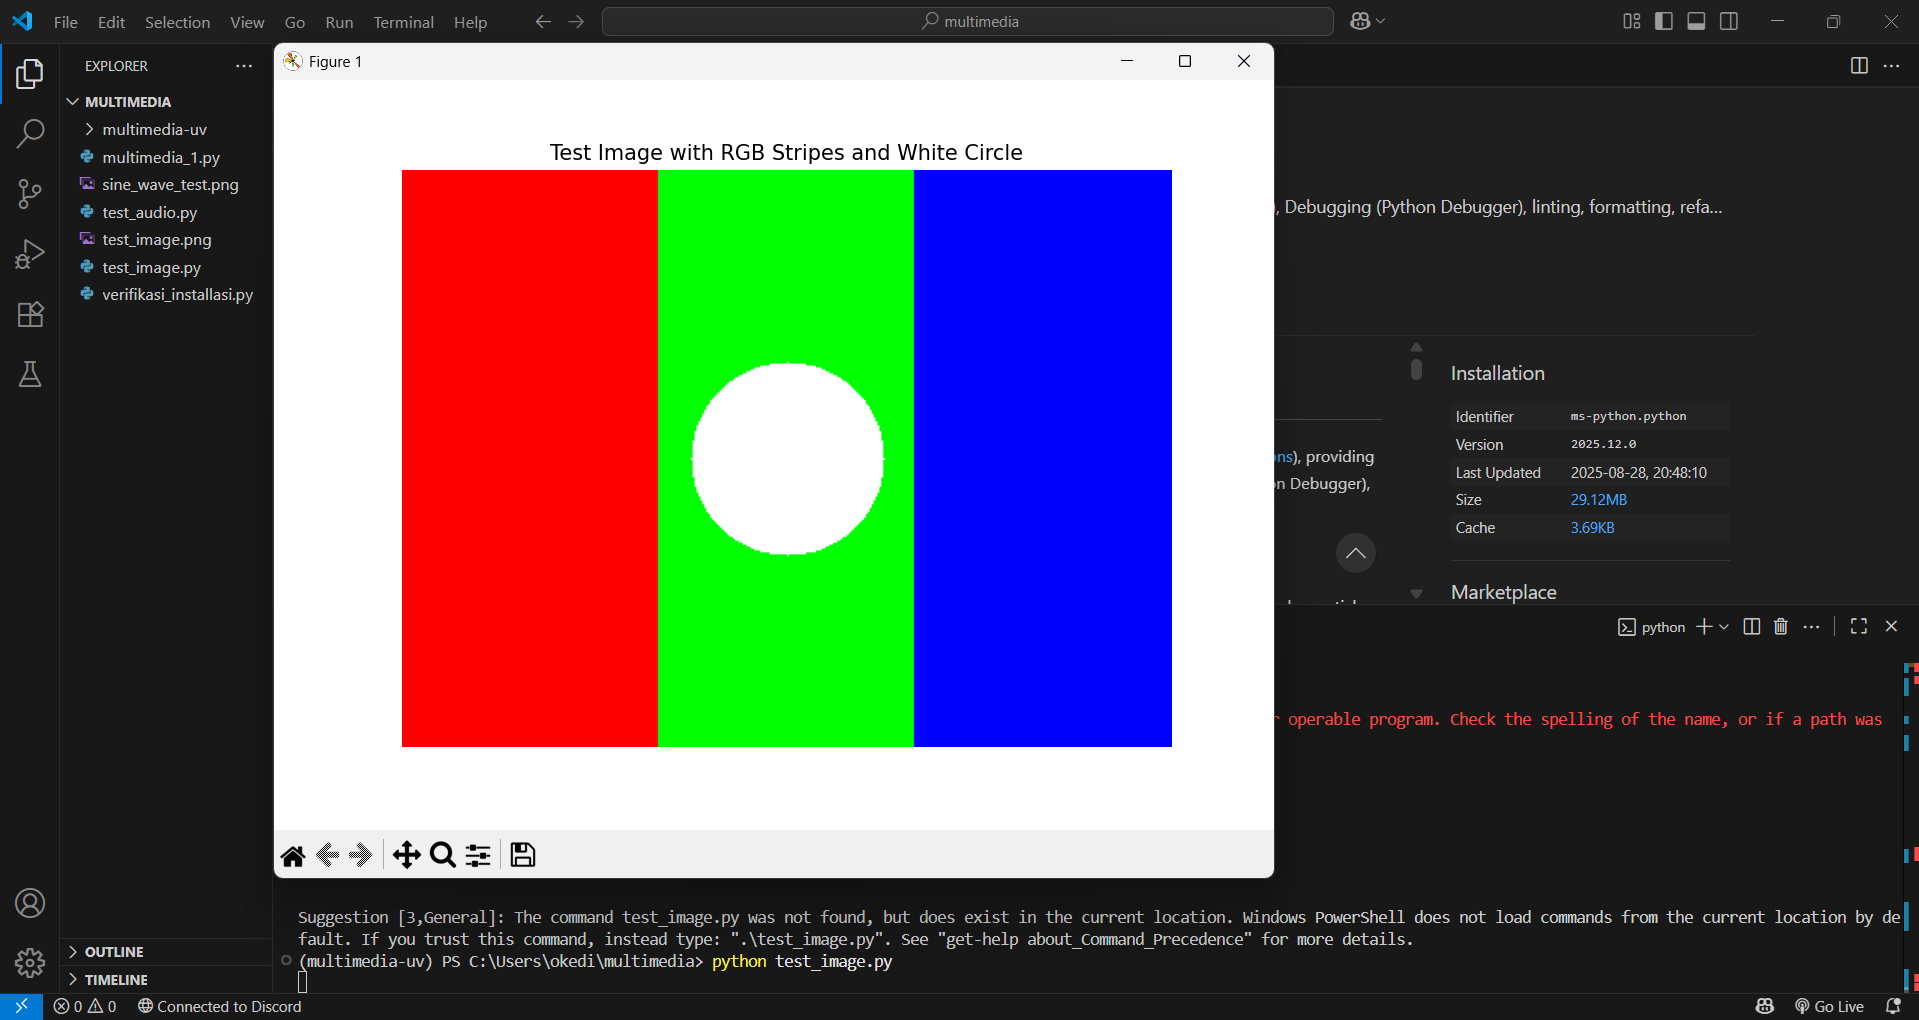
\includegraphics[width=0.7\textwidth]{Figure/ss10.png}
        \caption{Output dari script test image}
        \label{fig:contoh-gambar}
    \end{figure}
\end{itemize}

\subsection{Analisis dan Refleksi}
\textbf{Jawab pertanyaan berikut:}

\begin{enumerate}
    \item \textbf{Mengapa penting menggunakan environment terpisah untuk project multimedia?}
    
    \textit{Penting untuk menggunakan environment terpisah untuk setiap proyek multimedia. Hal ini dikarenakan masing-masing proyek biasanya membutuhkan library dan versi yang berbeda. Sebagai contoh, pada proyek 1 membutuhkan versi tertentu dari sebuah library, sementara proyek 2 memerlukan versi yang berbeda. Jika kedua proyek dijalankan dalam environment yang sama, versi library akan saling bertabrakan. Dengan membuat environment terpisah, setiap proyek bisa menggunakan versi library yang sesuai tanpa menimbulkan konflik atau error.}
    
    \item \textbf{Apa perbedaan utama antara conda, venv, dan uv? Mengapa Anda memilih tool yang Anda gunakan?}
    
    \textit{Menurut saya perbedaan antar conda, venv, dan uv terletak pada masing-masing fiturnya conda walaupun toolnya yang termasuk berat tetapi conda memiliki banyak paket yang sudah terinstall dan mudah digunakan untuk proyek multimedia, sedangkan venv adalah tool bawaan python yang ringan dan sederhana, namun memerlukan instalasi manual untuk setiap library. Sedangkan uv adalah tool yang lebih modern dan cepat dibandingkan venv, serta memiliki fitur tambahan seperti manajemen dependency yang lebih baik. Saya memakai uv dikarenakan uv lebih ringan dan cepat.}
    
    \item \textbf{Library mana yang paling sulit diinstall dan mengapa?}
    
    \textit{tadinya kesulitan install library dikarenakan saat melakukan instalasi saya salah memilih environment yang digunakan. tetapi sebenarnya dalam melakukan instalasi library itu sangat mudah}
    
    \item \textbf{Bagaimana cara mengatasi masalah dependency conflict jika terjadi?}
    
    \textit{Apabila ada library yang mengalami masalah versi, melakukan upgrade akan membuat UV secara otomatis memasang versi yang sesuai. Selain itu, perintah uv pip check dapat digunakan untuk melihat library mana yang memiliki konflik versi, sehingga bisa diperbaiki dengan menghapus atau memperbaruinya.}
    
    \item \textbf{Jelaskan fungsi dari masing-masing library yang berhasil Anda install!}
    \begin{itemize}
    \item \textbf{librosa}: Analisis audio/musik dan ekstraksi data dari file audio.
    \item \textbf{soundfile}: Membaca dan menulis file audio.
    \item \textbf{scipy}: Algoritma untuk optimisasi, aljabar linear, FFT, dan statistik.
    \item \textbf{cv2 (OpenCV)}: Computer vision untuk memproses dan menganalisis gambar/video.
    \item \textbf{PIL (Pillow)}: Manipulasi gambar, seperti resize, crop, filter, dan konversi format.
    \item \textbf{scikit-image}: Pengolahan citra, termasuk filter dan transformasi.
    \item \textbf{matplotlib}: Membuat grafik, plot, dan visualisasi data.
    \item \textbf{moviepy}: Mengedit dan memproses video.
    \item \textbf{numpy}: Komputasi numerik dengan array/matriks.
    \item \textbf{pandas}: Analisis dan manipulasi data tabel.
    \item \textbf{jupyter (notebook)}: Notebook interaktif untuk kode, teks, grafik, dan eksekusi.
\end{itemize}

\end{enumerate}

\subsection{Troubleshooting}
\textbf{Dokumentasikan masalah yang Anda hadapi (jika ada) dan cara mengatasinya:}

\begin{itemize}
    \item \textbf{Masalah 1:} \textit{Penggunaan Which yang salah, seharusnya menggunakan Where. Saat saya menjalankan perintah, saya mendapatkan error yang menyatakan bahwa 'Which' tidak ditemukan.}
    
    \textbf{Solusi:} \textit{Setelah saya bertanya melalui GPT, GPT sendiri menyuruh untuk menggunakan where yang dimana where tersebut merupakan perintah yang digunakan untuk windows sedangkan untuk where merupakan perintah yang ada di Linux/Macbook. Saya memperbaiki perintah dengan mengganti 'Which' menjadi 'Where' dan menjalankannya kembali.}
    
    \item \textbf{Masalah 2:} \textit{Salah dalam melakukan instalasi library}
    
    \textbf{Solusi:} \textit{Ketika saya bertanya kepada GPT ternyata pip yang berada pada multimedia-ev tidak ada, kemudian saya melakukan penginstalan pip secara manual, lalu saya menjalankan perintah menggunakan -m supaya agar menjalakan module sebagai script.}
\end{itemize}

\section{Export Environment untuk Reproduksi}
Sebagai langkah terakhir, export environment Anda agar dapat direproduksi:

\subsection{Untuk Conda}
\begin{lstlisting}[language=bash, caption=Export conda environment]
conda env export > environment.yml
\end{lstlisting}

\subsection{Untuk venv/uv}
\begin{lstlisting}[language=bash, caption=Export pip requirements]
pip freeze > requirements.txt
\end{lstlisting}

\textbf{Copy-paste isi file environment.yml atau requirements.txt di sini:}

\begin{lstlisting}[caption=Environment/Requirements file]
anyio==4.10.0
argon2-cffi==25.1.0
argon2-cffi-bindings==25.1.0
arrow==1.3.0
asttokens==3.0.0
async-lru==2.0.5
attrs==25.3.0
audioread==3.0.1
babel==2.17.0
beautifulsoup4==4.13.5
bleach==6.2.0
certifi==2025.8.3
cffi==1.17.1
charset-normalizer==3.4.3
colorama==0.4.6
comm==0.2.3
contourpy==1.3.2
cycler==0.12.1
debugpy==1.8.16
decorator==5.2.1
defusedxml==0.7.1
exceptiongroup==1.3.0
executing==2.2.0
fastjsonschema==2.21.2
fonttools==4.59.2
fqdn==1.5.1
h11==0.16.0
httpcore==1.0.9
httpx==0.28.1
idna==3.10
imageio==2.37.0
imageio-ffmpeg==0.6.0
ipykernel==6.30.1
ipython==8.37.0
ipywidgets==8.1.7
isoduration==20.11.0
jedi==0.19.2
Jinja2==3.1.6
joblib==1.5.2
json5==0.12.1
jsonpointer==3.0.0
jsonschema==4.25.1
jsonschema-specifications==2025.4.1
jupyter==1.1.1
jupyter-console==6.6.3
jupyter-events==0.12.0
jupyter-lsp==2.3.0
jupyter_client==8.6.3
jupyter_core==5.8.1
jupyter_server==2.17.0
jupyter_server_terminals==0.5.3
jupyterlab==4.4.6
jupyterlab_pygments==0.3.0
jupyterlab_server==2.27.3
jupyterlab_widgets==3.0.15
kiwisolver==1.4.9
lark==1.2.2
lazy_loader==0.4
librosa==0.11.0
llvmlite==0.44.0
MarkupSafe==3.0.2
matplotlib==3.10.5
matplotlib-inline==0.1.7
mistune==3.1.4
moviepy==2.2.1
msgpack==1.1.1
nbclient==0.10.2
nbconvert==7.16.6
nbformat==5.10.4
nest-asyncio==1.6.0
networkx==3.4.2
notebook==7.4.5
notebook_shim==0.2.4
numba==0.61.2
numpy==2.2.6
opencv-python==4.12.0.88
overrides==7.7.0
packaging==25.0
pandas==2.3.2
pandocfilters==1.5.1
parso==0.8.5
pillow==11.3.0
platformdirs==4.4.0
pooch==1.8.2
proglog==0.1.12
prometheus_client==0.22.1
prompt_toolkit==3.0.52
psutil==7.0.0
pure_eval==0.2.3
pycparser==2.22
Pygments==2.19.2
pyparsing==3.2.3
python-dateutil==2.9.0.post0
python-dotenv==1.1.1
python-json-logger==3.3.0
pytz==2025.2
pywin32==311
pywinpty==3.0.0
PyYAML==6.0.2
pyzmq==27.0.2
referencing==0.36.2
requests==2.32.5
rfc3339-validator==0.1.4
rfc3986-validator==0.1.1
rfc3987-syntax==1.1.0
rpds-py==0.27.1
scikit-image==0.25.2
scikit-learn==1.7.1
scipy==1.15.3
Send2Trash==1.8.3
six==1.17.0
sniffio==1.3.1
soundfile==0.13.1
soupsieve==2.8
soxr==0.5.0.post1
stack-data==0.6.3
terminado==0.18.1
threadpoolctl==3.6.0
tifffile==2025.5.10
tinycss2==1.4.0
tomli==2.2.1
tornado==6.5.2
tqdm==4.67.1
traitlets==5.14.3
types-python-dateutil==2.9.0.20250822
typing_extensions==4.15.0
tzdata==2025.2
uri-template==1.3.0
urllib3==2.5.0
wcwidth==0.2.13
webcolors==24.11.1
webencodings==0.5.1
websocket-client==1.8.0
widgetsnbextension==4.0.14
\end{lstlisting}

\section{Kesimpulan}
\textbf{Tuliskan kesimpulan Anda mengenai:}
\begin{itemize}
    \item Pengalaman setup Python environment untuk multimedia
    \item Persiapan untuk project multimedia selanjutnya
    \item Saran untuk mahasiswa lain yang akan melakukan setup serupa
\end{itemize}

\textit{Pengalaman saya dalam melakukan setup python environment adalah lumayan cukup pusing, terutama dalam mengatasi permasalah-permasalahan tadi. Namun, dengan bantuan dokumentasi dan forum online, saya berhasil menyelesaikan masalah yang ada. Untuk project multimedia selanjutnya, saya akan lebih berhati-hati dalam dalam mengikuti langkah-langkah dan memperhatikan dependensi yang digunakan dan mencoba untuk menggunakan virtual environment agar lebih terisolasi. Saran saya untuk mahasiswa lain yang akan melakukan setup serupa adalah untuk selalu berhati-hati dalam mengikuti langkah-langkah yang ada sehingga tidak terjadi kesalahan yang bisa mempersulit proses setup.}

\section{Referensi}
Referensi Troubleshooting \href{https://chatgpt.com/share/68b1b4fe-8fac-800d-b4e2-c8d4d330802c}{Chat GPT - Open AI}

\newpage
\bibliographystyle{IEEEtran}
\bibliography{Referensi}
\end{document}